% Use pdflatex.exe -synctex=1 -interaction=nonstopmode "graphparsing".tex
% For bibliography use BibTex
\documentclass[sigconf,edbt]{acmart-edbt2018}

\usepackage{graphicx}

\usepackage{caption}
\usepackage{subcaption}
%\usepackage{gnuplottex}
\usepackage{tikz}
\usepackage{mathtools}

\usepackage{graphicx}
\usepackage{hyperref}
\usepackage{textcomp}

\usepackage{algpseudocode}
\usepackage{algorithm}
\usepackage{algorithmicx}

\usepackage{booktabs} % For formal tables

% Copyright
\setcopyright{rightsretained}

% DOI
\acmDOI{}

% ISBN
\acmISBN{978-3-89318-078-3}

%Conference
\acmConference[EDBT 2018]{21st International Conference on Extending Database Technology (EDBT)}{March 26-29, 2018}{Vienna, Austria} 
\acmYear{2018}

\settopmatter{printacmref=false, printccs=false, printfolios=false}

\pagestyle{plain} % removes running headers


\begin{document}
	
\newtheorem{mytheorem}{Theorem}
%\newtheorem{lemma}{Lemma}
\newtheorem{mydef}{Definition}

\algrenewcommand\algorithmicindent{0.5em}
\algnewcommand\algorithmicswitch{\textbf{switch}}
\algnewcommand\algorithmiccase{\textbf{case}}
\algnewcommand\algorithmicassert{\texttt{assert}}
\algnewcommand\Assert[1]{\State \algorithmicassert(#1)}
% New "environments"
\algdef{SE}[SWITCH]{Switch}{EndSwitch}[1]{\algorithmicswitch\ #1\ \algorithmicdo}{\algorithmicend\ \algorithmicswitch}
\algdef{SE}[CASE]{Case}{EndCase}[1]{\algorithmiccase\ #1}{\algorithmicend\ \algorithmiccase}

\algtext*{EndSwitch}
\algtext*{EndCase}
\algtext*{EndWhile}% Remove "end while" text
\algtext*{EndIf}% Remove "end if" text
\algtext*{EndFor}% Remove "end for" text
\algtext*{EndFunction}% Remove "end function" text

\newif\ifboldnumber
\newcommand{\boldnext}{\global\boldnumbertrue}


\title{Context-Free Path Querying by Matrix Multiplication}

\author{Rustam Azimov}
\affiliation{%
  \institution{Saint Petersburg State University}
  \streetaddress{7/9 Universitetskaya nab.}
  \city{St. Petersburg} 
  \state{Russia} 
  \postcode{199034}
}
\email{rustam.azimov19021995@gmail.com}

\author{Semyon Grigorev}
\affiliation{%
	\institution{Saint Petersburg State University}
	\streetaddress{7/9 Universitetskaya nab.}
	\city{St. Petersburg}
	\state{Russia}  
	\postcode{199034}
}
\email{Semen.Grigorev@jetbrains.com}

% The default list of authors is too long for headers}
% \renewcommand{\shortauthors}{B. Trovato et al.}
\renewcommand{\shortauthors}{}

\begin{abstract}
Graph data models are widely used in many areas, for example, bioinformatics, graph databases. One of the most common graph queries are navigational queries. The result of query evaluation is a set of implicit relations between nodes of the graph, i.e. paths in the graph. A natural way to specify these relations is by specifying paths using formal grammars over the alphabet of edge labels. An answer to a context-free path query in this approach is usually a set of triples $(A, m, n)$ such that there is a path from node $m$ to node $n$, whose labeling is derived from a non-terminal $A$ of the given context-free grammar. This type of queries is evaluated using the \textit{relational query semantics}. Another example of path query semantics is \textit{single-path query semantics} which requires to present a single path from node $m$ to node $n$, whose labeling is derived from a non-terminal $A$ for all triples $(A, m, n)$ evaluated using relational query semantics. There is a number of algorithms for query evaluation which use these semantics but all of them perform poorly on a large graphs. One of the most common technique for efficient big data processing is GPGPU, but these algorithms do not allow to use this technique efficiently. In this paper we show how the context-free path query evaluation using these query semantics can be reduced to the calculation of the matrix transitive closure. Also we propose an algorithm for context-free path query evaluation which uses relational query semantics and is based on matrix operations that make it possible to speed up computations by using GPGPU.
\end{abstract}

\keywords{Transitive closure, CFPQ, graph databases, context-free grammar, GPGPU, matrix multiplication}

\maketitle

\chapter*{Введение}                         % Заголовок
\addcontentsline{toc}{chapter}{Введение}    % Добавляем его в оглавление
\textbf{Актуальность работы}

Статический анализ исходного кода является известной техникой  получения знаний о программе без её исполнения ~\cite{StaticCodeAnalysis3,StaticCodeAnalysis2,StaticCodeAnalysis1}. Статический анализ является неотъемлемой частью многих процессов, связанных с разработкой программного обеспечения (ПО), и может использоваться, например, для упрощения работы с кодом с помощью подсветки синтаксиса языка в программах, навигации по коду, реализации контекстных подсказок. Более того, статический анализ используется для обнаружения ошибок на ранних стадиях разработки, до запуска программы, а также для поиска различных семантических ошибок, которые не могут быть определены обычным синтаксическим анализом.  Также, статический анализ используется при решении задач трансформации исходного кода и реинжиниринге~\cite{reengANT}. Однако во многих языках программирования имеются конструкции, которые существенно затрудняют статический анализ. 

Например, широко используются динамические встроенные языки --- приложение, созданное на одном языке, генерирует программу на другом языке и передаёт её на выполнение в соответствующее окружение. Примерами могут служить динамические SQL-запросы к базам данных из приложений на Java, С++, С\#, формирование HTML-страниц в PHP-приложениях~\cite{DSQLISO,JSP,PHPmySQL}. Генерируемый код собирается из строк таким образом, чтобы в момент выполнения результирующая строка представляла собой корректную программу. Примеры использования встроенных языков представлены в листингах~\ref{lst:dsql1},~\ref{lst:JsJava} и~\ref{lst:PhPSqlHtml}. Следует отметить, что одна программа может генерировать код на нескольких языках (см. листинг~\ref{lst:PhPSqlHtml}). При этом возможно получение частей кода из разных источников (например, учитывать текстовый ввод пользователя, что часто используется для задания фильтров при конструировании SQL-запросов). Использование динамически формируемых программ  позволяет избежать дополнительных накладных расходов, присущих таким технологиям, как ORM\footnote{ORM или Object-Relational Mapping --- технология программирования, которая связывает базы данных с концепциями объектно-ориентированных языков программирования~\cite{ORM}.}, и достичь высокой производительности. Благодаря этому использование динамически генерируемых программ получило широкое распространение и применяется до сих пор. Вместе с этим, несмотря на появление новых технологий, динамическая генерация SQL-запросов активно используется и в настоящее время~\cite{DSQLInActiveUse}.

\fvset{frame=lines,framesep=5pt,fontsize=\small}\

\begin{listing}
    \begin{pyglist}[language=sql,numbers=left,numbersep=5pt]

CREATE PROCEDURE [dbo].[MyProc]  @TABLERes   VarChar(30)
AS
    EXECUTE ('INSERT INTO ' + @TABLERes + ' (sText1)' +
             ' SELECT ''Additional condition: '' + sName' +
             ' from #tt where sAction = ''1000000''')
GO
    \end{pyglist}
\caption{Код с использованием динамического SQL}
\label{lst:dsql1}
\end{listing} 
 
\fvset{frame=lines,framesep=5pt}
\begin{listing}
    \begin{pyglist}[language=java,numbers=left,numbersep=5pt]
import javax.script.*;  
public class InvokeScriptFunction {  
    public static void main(String[] args) throws Exception {  
        ScriptEngineManager manager = new ScriptEngineManager();  
        ScriptEngine engine = manager.getEngineByName("JavaScript");  
        // JavaScript code in a String  
        String script = 
            "function hello(name) { print('Hello, ' + name); }";  
        // evaluate script  
        engine.eval(script);  
        // javax.script.Invocable is an optional interface.  
        // Check whether your script engine implements or not!  
        // Note that the JavaScript engine implements
        // Invocable interface.  
        Invocable inv = (Invocable) engine;  
        // invoke the global function named "hello"  
        inv.invokeFunction("hello", "Scripting!!" );  
    }  
}
    \end{pyglist}
\caption{Вызов JavaScript из Java}
\label{lst:JsJava}
\end{listing}


\fvset{frame=lines,framesep=5pt}
\begin{listing}
    \begin{pyglist}[language=php,numbers=left,numbersep=5pt]

<?php
    // Embedded SQL
    $query = 'SELECT * FROM ' . $my_table; 
    $result = mysql_query($query);
    
    // HTML markup generation
    echo "<table>\n";
    while ($line = mysql_fetch_array($result, MYSQL_ASSOC)) {
        echo "\t<tr>\n";    
        foreach ($line as $col_value) {
            echo "\t\t<td>$col_value</td>\n";
        }
        echo "\t</tr>\n";
    }
    echo "</table>\n";
?>
    \end{pyglist}
\caption{Использование нескольких встроенных в PHP языков (MySQL, HTML)}
\label{lst:PhPSqlHtml}
\end{listing}



Динамически формируемые выражения часто конструируются с помощью таких операций, как конкатенация в циклах или условных предложениях, или в рекурсивных процедурах. Это затрудняет статический анализ и приводит к получению множества возможных значений для каждого выражения в момент выполнения. Вследствие этого фрагменты динамически формируемого кода воспринимаются компилятором исходного языка как простые строки, не подлежащие дополнительному анализу, а это, в свою очередь, приводит к высокой вероятности возникновения ошибок во время выполнения программы. В худшем случае такая ошибка не приведёт к прекращению работы приложения, что указало бы на проблемы, однако целостность данных при этом может оказаться нарушена. Более того, использование динамически формируемых выражений затрудняет не только разработку информационных систем, так и также и реинжиниринг, поскольку в последнем случае важно автоматизировать перенос системы на новые зыки и платформы, что невозможно без качественного статического анализа. Например, при наличии в коде приложения динамически формируемых SQL-запросов нельзя точно ответить на вопрос о том, с какими элементами базы данных не взаимодействует система, и удалить их. При переносе такой системы на другую СУБД необходимо гарантировать, что для всех динамически формируемых выражений значение в момент выполнения будет корректным кодом на языке новой СУБД~\cite{JSquash}. Следует отметить, что отсутствие статического анализа динамически формируемых программ не позволяет реализовывать для них стандартную функциональность интегрированных сред разработки (Integrated Development Environment, IDE) --- подсветку синтаксиса и автодополнение, рефакторинг кода и т.д. Такая функциональность значительно упрощает процесс разработки и отладки приложений и полезна не только для основного языка, но и для встроенных языков. 

Для решения всех перечисленных выше задач необходимы инструменты, проводящие статический анализ динамически формируемых программ. Такой анализ может дать существенную информацию о таких программах, поскольку редко встречается ситуация полной динамической неопределённости (например, при создании динамических программ исключительно на основе пользовательского ввода). В большинстве случаев, имея программу, генерирующую динамические вставки, с помощью статического анализа можно получить достаточно информации для решения поставленных выше задач. Решению этой проблемы и посвящена данная диссертационная работа. 


\textbf{Степень разработанности темы}

Существуют классические исследования, посвященные разработке компиляторов --- работы А.~Ахо~\cite{Dragon}, А.~Брукера~\cite{CompilerCompiler}, С.~Джонсона~\cite{yaccBook},  Б.К.Мартыненко~\cite{Martinenko1, Martinenko2}  и др.  Однако содержащиеся там алгоритмы синтаксического анализа не могут быть применены к решению задачи анализа динамически формируемых программ, поскольку предназначены для обработки входных данных, представимых в видн линейной последовательности символов, а такое представление динамически формируемых программ не всегда возможно.

Методы обобщённого синтаксического анализа, лежащие в основе данной работы, изложены в трудах таких учёных как Масару Томита (Masaru Tomita)~\cite{Tomita}, Элизабет Скотт (Elizabeth Scott) и Адриан Джонстон (Adrian Johnstone)~\cite{RNGLR,RIGLR} из университета Royal Holloway (Великобритания), Ян Рекерс (Jan Rekers, University of Amsterdam)~\cite{SPPF}, Элко Виссер (Eelco Visser)~\cite{RNGLRSyntaxerror2,RNGLRSyntaxerror3} и других.

Анализу динамически формируемых строковых выражений посвящены работы таких зарубежных учёных как Кюнг-Гу Дох (Kyung-Goo Doh)~\cite{LrAbstract1,LrAbstract2,LRAbstractParsingSema}, Ясухико Минамиде (Minamide Yasuhiko)~\cite{PHPSA}, Андерс Мёллер (Anders M{\o}ller)~\cite{JSA} и отечественных учёных А.А.~Бреслава~\cite{Alvor1,Alvor2} и других. Хорошо изучены вопросы проверки корректности динамически формируемых выражений и поиска фрагментов кода, уязвимых для SQL-инъекций~\cite{SQLInjection,Dasgupta:2009:SAF:1546683.1547548}. Однако данные работы исследуют отдельные аспекты проблемы статического анализа динамически формируемых программ, оставляя в стороне создание готовых алгоритмов (в частности, не строят структурное представление анализируемых программ). В связи с этим возникают проблемы масштабируемости данных результатов, например, создание на их основе более сложных видов статического анализа.

Так же важным является предоставление компонентов, упрощающих создание новых инструментов для решения конкретных задач. Данных подход хорошо исследован в области разработки компиляторов, где широкое распространение получили генераторы анализаторов и пакеты стандартных библиотек (работы А.~Ахо~\cite{Dragon}, А.~Брукера~\cite{CompilerCompiler}, С.~Джонсона~\cite{yaccBook} и др.). 

В работах отечественных учёных М.Д.~Шапот и Э.В.~Попова~\cite{DynamicDSQLTranslation}, а так же зарубежных учёных Антони Клеви (Anthony Cleve), Жан-Люк Эно (Jean-Luc Hainaut)~\cite{DSQLReverseEngineering}, Йост Виссер (Joost Visser)~\cite{DSQLQualityMesure} и других рассматриваются различные аспекты реинжиниринга информационных систем, использующих встроенные SQL-запросы, однако не формулируется общего метода для решения таких задач. Этот вопрос также не затрагивается в классических работах, посвященных реинжиниригу~\cite{SoftwareReeng1, reengANT, SoftwareReeng2, SoftwareReeng3}. Однако разработка такого метода является актуальной задачей.

Таким образом, актуальной является задача дальнейшего исследования статического анализа динамически формируемых строковых выражений. Кроме этого важным является решение вопросов практического применения средств анализа динамически формируемого кода: упрощение разработки инструментов анализа и создание методов их применения в реинжиниринге программного обеспечения.
\textbf{Объект исследования}

Объектом исследования являются методы, алгоритмы и программные средства обработки динамически формируемых программ, а также задача реинжиниринга информационных систем.

\textbf{Цель и задачи диссертационной работы}

\textbf{Целью} данной работы является создание комплексного подхода к статическому синтаксическому анализу динамически формируемых программ.

Достижение поставленной цели обеспечивается решением следующих \textbf{задач}.
\begin{enumerate}
    \item Разработать универсальный алгоритм синтаксического анализа динамически формируемых программ, не зависящий от целевого языка программирования и допускающий реализацию различных видов статического анализа. 
    \item Создать архитектуру инструментария для автоматизации разработки программных средств статического анализа динамически формируемых программ.
    \item Создать метод реинжиниринга динамически формируемых программ.
\end{enumerate}

\textbf{Методология и методы исследования}

Методология исследования основана на подходе к спецификации и анализу формальных языков, активно развивающемуся с 50-х годов 20-го века (см., например, работы Н. Хомского~\cite{chomskyMethod ,chomskySyntactic}). В последствии этот подход получил широкое распространение в областях, связанных с обработкой языков программирования.
Основными элементами данного подхода являются алфавит и грамматика языка, разбиение автоматической обработки языка на выполнение таких шагов как лексический, синтаксический и семантический анализ. Решаемые в связи с этим задачи связаны с поиском эффективных алгоритмов, выполняющих эти шаги. 

В работе применяется алгоритм обобщённого восходящего синтаксического анализа RNGLR~\cite{RNGLR}, созданный Элизабет Скотт (Elizabeth Scott) и Адриан Джонстон (Adrian Johnstone) из университета Royal Holloway (Великобритания). Для компактного хранения леса вывода использовалась структура данных Shared Packed Parse Forest (SPPF), которую предложил Ян Рекерс (Jan Rekers, University of Amsterdam)~\cite{SPPF}.

Доказательство завершаемости и корректности предложенного алгоритма проводилось с применением теории формальных языков, теории графов и теории сложности алгоритмов. Приближение множества значений динамически формируемого выражения строилось в виде регулярного множества, описываемого с помощью конечного автомата.


\textbf{Положения, выносимые на защиту}
\begin{enumerate}
    \item Разработан алгоритм синтаксического анализа динамически формируемых программ, позволяющий обрабатывать произвольную регулярную аппроксимацию множества значений выражения в точке выполнения, реализующий эффективное управление стеком и гарантирующий конечность представления леса вывода. Доказана завершаемость и корректность предложенного алгоритма при обработке регулярной аппроксимации, представимой в виде произвольного конечного автомата без $\varepsilon$-переходов. 
    \item Создана архитектура инструментария для разработки программных средств статического анализа динамически формируемых программ.
    \item Разработан метод анализа и обработки динамически формируемых программ в проектах по реинжинирингу информационных систем. 
\end{enumerate}

\textbf{Научная новизна работы}

Научная новизна полученных в ходе исследования результатов заключается в следующем.

\begin{enumerate}

\item Алгоритм, предложенный в диссертации, отличается от аналогов (работы Андрея Бреслава~\cite{Alvor1, Alvor2}, Кюнг-Гу Дох~\cite{LrAbstract1, LrAbstract2}, Ясухико Минамиде~\cite{PHPSA}) возможностью построения компактной структуры данных, содержащей деревья вывода для всех корректных значений выражения. Это позволяет использовать результаты работы алгоритма для проведения более сложных видов анализа. Алгоритмы, представленные в (JSA~\cite{JSA}~\cite{Alvor1, Alvor2}, PHPSA~\cite{PHPSA}) предназначены только для проверки корректности выражений, основанной на решении задачи о включении одного языка в другой. Выполнение более сложных видов анализа, трансформаций или построения леса разбора не предполагается. 

\item Новизна представленной архитектуры заключается в том, что она позволяет создать платформу для разработки целевых инструментов, решающих широкий круг задач анализа динамически формируемого кода. Существующие архитектуры готовых инструментов (JSA, PHPSA, Alvor, Varis) предназначены для решения конкретных задач для определённых языков. Решение новых задач или поддержка других языков с помощью этих инструментов затруднены ввиду ограничений, накладываемых архитектурой и возможностями используемого алгоритма анализа. 

\item Метод анализа и обработки встроенного программного кода в проектах по реинжинирингу информационных систем предложен впервые. К.В.~Ахтырченко и Т.П.~Сорокваша отмечают~\cite{SoftwareReengMethods}, что существующие работы в области реинжиниринга программного обеспечения либо содержат высокоуровневые решения, не касающиеся деталей, важных при решении прикладных задач (например, работы К. Вагнера~\cite{SoftwareReeng3}, Х. Миллера~\cite{SoftwareReeng2}), либо являются набором подходов к решению конкретных задач (например, работы~\cite{SoftwareReeng1, reengANT, boulychev}). При этом, встроенный программный код часто не учитывается. С другой стороны, работы М.Д.~Шапот и Э.В.~Попова~\cite{DynamicDSQLTranslation}, С.Л.~Трошина~\cite{reengANT}, А.~Клеви~\cite{DSQLReverseEngineering}  посвящены решению конкретных задач обработки встроенного программного кода в контексте реинжиниринга информационных систем, но не предлагают обобщённого и масштабируемого метода.

\end{enumerate}


\textbf{Теоретическая и практическая значимость работы}

Теоретическая значимость диссертационного исследования заключается в разработке формального алгоритма синтаксического анализа динамически формируемого кода, решающего задачу построения конечного представления леса вывода, не решенную полностью ранее, а также в формальном доказательстве завершаемости и корректности разработанного алгоритма. 

На основе полученных в работе научных результатов был разработан инструментарий (Software Development Kit, SDK), предназначенный для создания средств статического анализа динамически формируемых программ. 
С использованием разработанного инструментария было реализовано расширение к инструменту ReSharper (ООО ``ИнтеллиДжей Лабс'', Россия), предоставляющее поддержку встроенного T-SQL в проектах на языке программирования C\# в среде разработки Microsoft Visual Studio. Так же было выполнено внедрение результатов работы в промышленный проект по переносу хранимого SQL-кода с MS-SQL Server 2005 на Oraclе 11gR2 (ЗАО ``Ланит-Терком'', Россия). 

\textbf{Степень достоверности и апробация результатов}

Достоверность и обоснованность результатов исследования опирается на использование формальных методов исследуемой области, проведенные доказательства, рассуждения и эксперименты.

Основные результаты работы были доложены на ряде научных конференций: SECR-2012, SECR-2013, SECR-2014, TMPA-2014, Parsing@SLE-2013, Рабочий семинар ``Наукоемкое программное обеспечение'' при конференции PSI-2014. Доклад на SECR-2014 награждён премией Бертрана Мейера за лучшую исследовательскую работу в области программной инженерии. Дополнительной апробацией является то, что разработка инструментальных средств на основе предложенного алгоритма была поддержана Фондом содействия развитию малых форм предприятий в технической сфере (программа УМНИК~\cite{UMNIC}, проекты \textnumero~162ГУ1/2013 и \textnumero~5609ГУ1/2014).

\textbf{Публикации по теме диссертации}

Все результаты диссертации изложены в 7 научных работах, из которых 3~\cite{YCArticle,SELforIDEru,AbstractGLL}, содержащие основные результаты, опубликованы в журналах из ‘’Перечня российских рецензируемых научных журналов, в которых должны быть опубликованы основные научные результаты диссертаций на соискание ученых степеней доктора и кандидата наук’’, рекомендовано ВАК. 
1 работа~\cite{GLRAbsPars} индексируются Scopus. В работах, написанных в соавторстве, вклад автора определяется следующим образом.  В~\cite{Syrcose} С. Григорьеву принадлежит реализация ядра платформы YaccConstructor. В~\cite{SELforIDEru, AbstractGLL} и~\cite{SELforIDE} С. Григорьеву принадлежит постановка задачи, формулирование требований к разрабатываемым инструментальным средствам, работа над текстом. 
В~\cite{GLRAbsPars} автору принадлежит идея, описание и реализация анализа встроенных языков на основе RNGLR алгоритма.  В~\cite{YCArticle} С. Григорьеву принадлежит реализация инструментальных средств, проведение экспериментов, работа над текстом. В работе~\cite{RelaxedARNGLR} автору принадлежит алгоритм синтаксического анализа динамически формируемого кода.


\textbf{Структура работы}

Диссертация состоит из введения, шести глав, заключения и построена следующим образом. В первой главе приводится обзор области исследования. Рассматриваются подходы к анализу динамически формируемых строковых выражений и соответствующие инструменты. Описывается алгоритм обобщённого восходящего синтаксического анализа RNGLR, взятый за основу в диссертационной работе. Также описываются проекты YaccConstructor и ReSharper SDK, использованные для реализации предложенного в работе инструментария. Во второй главе формализуется основная задача исследования и излагается решающий её алгоритм синтаксического анализа регулярных множеств. Приводится доказательство завершаемости и корректности представленного алгоритма, приводятся примеры. В третьей главе описывается инструментальный пакет YC.SEL.SDK, разработанного на основе алгоритма, описанного во второй главе и предназначеного для разработки инструментов анализа динамически формируемых программ. Описывается архитектура компонентов и особенности их реализации. Также описывается YC.SEL.SDK.ReSharper --- ``обёртка'' для YC.SEL.SDK, позволяющая создавать расширения к ReSharper для поддержки встроенных языков. В четвёртой главе описывается метод реинжиниринга встроенного программного кода.  В пятой главе приводятся результаты экспериментального исследования разработанного алгоритма и инструмента YC.SEL.SDK. Шестая глава содержит результаты сравнения и соотнесения полученных результатов с  существующими аналогами.

\textbf{Благодарности}

А.Н.Терехову, работкникам и администрации компании ЗАО ``Ланит-Терком'' за создания условий для изучения данной темы (организация проектов по реинжинирингу). Я.А.Кириленко за погружение в тему исследования и руководство на начальных этапах. Д.Ю.Булычеву за помощь в уточнении постановки задачи исследования и в написании статей. Студентам и аспирантам кафедры системного программирования Дмитрию Авдюхину, Анастасии Рагозиной, Екатерине Вербицкой, Марине Полубеловой, Иванову Андрею за помощь в реализации предложенных идей и проведение экспериментов. Отдельную благодарность  хочется выразить компании ООО ``ИнтеллиДжей Лабс'' и Андрею Иванову за поддержку исследований. Также хочется поблагодарить А.К.Петренко и В.М.Ицыксона, а также сотрудников ИСП РАН за ценные вопросы и комментарии к работе, позволившие уточнить ряд формулировок и улучшить изложение результатов. 

\section{Preliminaries} \label{section_preliminaries}
In this section, we introduce the basic notions used throughout the paper.

Let $\Sigma$ be a finite set of edge labels. Define an \textit{edge-labeled directed graph} as a tuple $D = (V, E)$ with $V$ is a set of nodes and $E \subseteq V \times \Sigma \times V$ is a directed edge-relation.  For a path $\pi$ in a graph $D$ we denote $l(\pi)$ --- the unique word obtained by concatenating the labels of the edges along the path $\pi$. Also, we write $n \pi m$ to indicate that a path $\pi$ starts at node $n \in V$ and ends at node $m \in V$.

According to Hellings~\cite{hellingsRelational}, we deviate from the usual definition of a context-free grammar in \textit{Chomsky Normal Form}~\cite{chomsky} by not including a special start non-terminal, which will be specified in the queries to the graph. Since every context-free grammar can be transformed into an equivalent one in Chomsky Normal Form and checking that an empty string is in the language is trivial, then it is sufficient to only consider grammars of the following type. A \textit{context-free grammar} is 3-tuple $G = (N, \Sigma, P)$ where $N$ is a finite set of non-terminals, $\Sigma$ is a finite set of terminals, and $P$ is a finite set of productions of the following forms:

\begin{itemize}
    \item $A \rightarrow B C$, for $A,B,C \in N$,
    \item $A \rightarrow x$, for $A \in N$ and $x \in \Sigma$.   
\end{itemize}

Note that we omit the rules of the form $A \rightarrow \varepsilon$, where $\varepsilon$ denotes an empty string. This does not limit the applicability of further algorithms because checking that an empty string belongs to the context-free language in Chomsky normal form is trivial and only the empty paths $m \pi m$ correspond to an empty string $\varepsilon$.

We use the conventional notation $A \xrightarrow{*} w$ to denote that the string $w \in \Sigma^*$ can be derived from a non-terminal $A$ by some sequence of applying the production rules from $P$. The \textit{language} of a grammar $G = (N,\Sigma,P)$ with respect to a start non-terminal $S \in N$ is defined by $L(G_S) = \{w \in \Sigma^*~|~S \xrightarrow{*} w\}$.

For a given graph $D = (V, E)$ and a context-free grammar $G = (N, \Sigma, P)$, we define \textit{context-free relations} $R_A \subseteq V \times V$, for every $A \in N$, such that $R_A = \{(n,m)~|~\exists n \pi m~(l(\pi) \in L(G_A))\}$.

We define a binary operation on arbitrary subsets $N_1 , N_2$ of $N$ with respect to a context-free grammar $G = (N, \Sigma, P)$ as $N_1 \cdot N_2 = \{A~|~\exists B \in N_1, \exists C \in N_2 \text{ such that }(A \rightarrow B C) \in P\}.$

Using this binary operation as a multiplication on arbitrary subsets of $N$ and union of sets as an addition, we can define a \textit{matrix multiplication}, $a \cdot b = c$, where $a$ and $b$ are matrices of the suitable size that have subsets of $N$ as elements, as $c_{i,j} = \bigcup^{n}_{k=1}{a_{i,k} \cdot b_{k,j}}$.

We define the \textit{transitive closure} of a square matrix $a$ as $a^+ = a^{(1)} \cup a^{(2)} \cup \cdots$ where $a^{(i)} = a^{(i-1)} \cup (a^{(i-1)} \cdot a^{(i-1)})$, $i \ge 2$ and $a^{(1)} = a$.
\section{Related works} \label{section_related}
The regular language constrained path querying is widely used for graph analysis~\cite{abiteboul1997regular,fan2011adding,nole2016regular,reutter2017regular}.

There are a number of solutions~\cite{azimov2018context,hellingsRelational,GraphQueryWithEarley,RDF} for context-free path query evaluation w.r.t. the relational query semantics, which employ such parsing algorithms as CYK~\cite{kasami,younger} or Earley~\cite{Grune}. Other examples of path query semantics are \textit{single-path} and \textit{all-path query semantics}. The all-path query semantics requires presenting all possible paths from node $m$ to node $n$ whose labeling is derived from a nonterminal $A$ for all triples $(A, m, n)$ evaluated using the relational query semantics. While the single-path query semantics requires presenting only one such a path for all the node-pairs $(m, n)$. Hellings~\cite{hellingsPathQuerying} presented algorithms for the context-free path query evaluation using the single-path and the all-path query semantics. If a context-free path query w.r.t. the all-path query semantics is evaluated on cyclic graphs, then the query result can be an infinite set of paths. For this reason, in~\cite{hellingsPathQuerying}, annotated grammars are proposed as a possible solution.

In~\cite{GLL}, the algorithm for context-free path query evaluation w.r.t. the all-path query semantics is proposed. This algorithm is based on the generalized top-down parsing algorithm~---~GLL~\cite{scott2010gll}. This solution uses derivation trees for the result representation which is more native for grammar-based analysis. The algorithms in~\cite{GLL,hellingsPathQuerying} for the context-free path query evaluation w.r.t. the all-path query semantics can also be used for query evaluation using the relational and the single-path semantics.

Hellings~\cite{hellingsRelational} presented an algorithm for the context-free path query evaluation using the relational query semantics. According to Hellings, for a given graph $D = (V, E)$ and a grammar $G = (N, \Sigma, P)$ the context-free path query evaluation w.r.t. the relational query semantics reduces to a calculation of the context-free relations $R_A$. Thus, in this work, we focus on the calculation of conjunctive relations which are similar to the context-free relations.

There is an algorithm~\cite{zhang2017context} for path querying with linear conjunctive grammars and relational query semantics. These grammars have no more than one nonterminal in each conjunct of the rule. The possibility of creating an algorithm for path query evaluation w.r.t. conjunctive grammars of an arbitrary form is an open problem since the linear conjunctive grammars are known to be strictly less powerful than the arbitrary conjunctive grammars~\cite{okhotinConjAndBool}.
\section{Relaxed Parsing of Regular Sets}

The input of the algorithm (see Algorithm~\ref{parsing}) is a reference grammar $G$ with alphabet of terminal symbols $T$ 
and a finite non-deterministic automaton $(Q, \Sigma, \delta, q_0, q_f)$ with a single start state $q_0$, single final state $q_f$ 
and no $\epsilon$-transitions, where $\Sigma \subseteq T$~--- alphabet of input symbols, $Q$~--- alphabet of states, 
$\delta$~--- transition relation. RNGLR parser tables and some accessory information (called $parserSource$ in pseudocode) 
are generated for the grammar $G$. 

The general idea of the algorithm is to traverse the automaton graph and sequentially construct GSS, similarly to RNGLR.
However, as we deal with a graph instead of a linear stream, the next symbol turns into the \emph{set of terminals} on the 
all outgoing edges of current vertex. This results in a a different semantics of pushing and reducing (see line~5, 
Algorithm~\ref{processVertex}, and lines~8 and~20, Algorithm~\ref{gss_construction}). We use queue $\mathcal Q$ to control the 
order of automaton graph vertices processing. Every time a new GSS vertex is added, all zero-reductions have to be performed 
and then new tokens have to be shifted, so a corresponging graph vertex has to be enqueueed for further processing. 
Addition of new GSS edge can produce reductions to handle, so the graph vertex at the tail of the added edge has 
also to be enqueueed (see Algorithm~\ref{gss_construction}). Reductions are applied along the paths in GSS, and if we add
a new edge to some tail vertex, which was already presented in GSS, we also have to recalculate all \emph{passing} reductions
(see \emph{applyPassingReductions} function in Algorithm~\ref{processVertex}).

Likewise RNGLR, we associate GSS vertices with positions in the input,
and, in our case, a position coinsides with some state of the input automaton. We construct some
inner data structure (referred to as inner graph) by copying input automaton graph and 
extending each its vertex with the following collections: 

\begin{itemize}
  \item \emph{processed}: GSS vertices, for which all the pushes were processed. 
   This set aggregates all GSS vertices, associated with inner graph vertex.
  \item \emph{unprocessed}: GSS vertices, for which all the pushes are to be processed. 
   This set is analogous to $\mathcal{Q}$ of original RNGLR.
  \item \emph{reductions}: a queue, which is analogous to $\mathcal{R}$ of original RNGLR: 
   all reductions to be processed.
  \item \emph{passingReductionsToHandle}: pairs of GSS vertex and GSS edge to apply 
   passing reductions along them.
\end{itemize}

Besides parser $state$ and $level$ (which is equal to the input automaton state), 
a collection of \emph{passing reductions} is stored in a GSS vertex. Passing reduction is a 
triplet $(startV, N, l)$, representing reductions, whose path contains given GSS vertex. 
This triplet is similar to one describing reduction, where $l$ is a remaining length of the path. 
Passing reductions are stored for every vertex of the path (except for the first and the last) 
during path search in \emph{makeReductions} function (see Algorithm~\ref{processVertex}).

We inherit SPPF construction from the original RNGLR; in our case, 
derivation trees for strings, accumulated along the paths of the input automaton 
graph, are merged. 

\begin{algorithm}[!ht]
\begin{algorithmic}[1]
\caption{Parsing algorithm}
\label{parsing}
\Function{parse}{$grammar, automaton$}
  \State{$inputGraph \gets$ construct inner graph representation of $automaton$}
  \State{$parserSource \gets$ generate RNGLR parser tables for $grammar$}
  \If{$inputGraph$ contains no edges}
    \If{$parserSource$ accepts empty input} {report success}
    \Else { report failure}
    \EndIf
  \Else
    \State{\Call{addVertex}{$inputGraph.startVertex, startState$}}
    \State{$\mathcal{Q}.Enqueue(inputGraph.startVertex)$}
    \While{$Q$ is not empty}
      \State{$v \gets \mathcal{Q}.Dequeue()$}
      \State{\Call{makeReductions}{$v$}}
      \State{\Call{push}{$v$}}
      \State{\Call{applyPassingReductions}{$v$}}
    \EndWhile
    \If{$v_f.level = q_f$ and $v_f.state$ is accepting} {report success}
    \Else { report failure}
    \EndIf
  \EndIf
\EndFunction
\end{algorithmic}
\end{algorithm}

\begin{algorithm}[!ht]
\begin{algorithmic}[1]
\caption{Single-vertex processing}
\label{processVertex}
\Function{push}{$innerGraphV$}
  \State{$\mathcal{U} \gets$ copy $innerGraphV.unprocessed$}
  \State{clear $innerGraphV.unprocessed$}
  \ForAll{$v_{h}$ in $\mathcal{U}$}  
    \ForAll{$e$ in outgoing edges of $innerGraphV$}
      \State{$push \gets$ calculate next state by $v_{h}.state$ and the token on $e$}
      \State{\Call{addEdge}{$v_{h}, e.Target, push, false$}}
      \State{add $v_{h}$ in $innerGraphV.processed$}
    \EndFor
  \EndFor
\EndFunction

\Function{makeReductions}{$innerGraphV$}
  \While{$innerGraphV.reductions$ is not empty}
    \State{$(startV, N, l) \gets innerGraphV.reductions.Dequeue()$}
    \State{find the set of vertices $\mathcal{X}$ reachable from $startV$}
    \State{along the path of length ($l-1$), or $0$ if $l=0$;}
    \State{add $(startV, N, l-i)$ in $v.passingReductions$,}
    \State{where $v$ is an $i$-th vertex of the path}
    \ForAll{$v_{h}$ in $\mathcal{X}$}
      \State{$state_{t} \gets$ calculate new state by $v_{h}.state$ and nonterminal $N$}
      \State{\Call{addEdge}{$v_{h}, startV, state_{t}, (l=0)$}}
    \EndFor
  \EndWhile
\EndFunction

\Function{applyPassingReductions}{$innerGraphV$}
  \ForAll{$(v, edge)$ in $innerGraphV.passingReductionsToHandle$}
    \ForAll{$(startV, N, l) \gets v.passingReductions.Dequeue()$}
      \State{find the set of vertices $\mathcal{X}$,}
      \State{reachable from $edge$ along the path of length ($l-1$)}
      \ForAll{$v_{h}$ in $\mathcal{X}$}
        \State{$state_{t} \gets$ calculate new state by $v_{h}.state$ and nonterminal $N$}
        \State{\Call{addEdge}{$v_{h}, startV, state_{t}, false$}}
      \EndFor
    \EndFor
  \EndFor
\EndFunction
\end{algorithmic}
\end{algorithm}
 
\begin{algorithm}[!ht]
\begin{algorithmic}[1]
\caption{GSS construction}
\label{gss_construction}
\Function{addVertex}{$innerGraphV, state$}
  \If{$innerGraphV.processed$ or $innerGraphV.unprocessed$ contains\\
    vertex $v$ with state = $state$ }
    \State{\Return{($v, false$)}}
  \Else
    \State{$v \gets$ create new vertex for $innerGraphV$ with state $state$}
    \State{add $v$ in $innerGraphV.unprocessed$}
    \ForAll{$e$ in outgoing edges of $innerGraphV$}
      \State{calculate the set of zero-reductions by $v$}
      \State{and the token on $e$ and add them in $innerGraphV.reductions$}
    \EndFor
    \State{\Return{$(v, true$)}}
  \EndIf
\EndFunction

\Function{addEdge}{$v_{h}, innerGraphV, state_{t}, isZeroReduction$}
  \State{$(v_{t}, isNew) \gets$ \Call{addVertex}{$innerGraphV, state_{t}$}}
  \If{GSS does not contain edge from $v_{t}$ to $v_{h}$}
    \State{$edge \gets$ create new edge from $v_{t}$ to $v_{h}$}
    \State{$\mathcal{Q}.Enqueue(innerGraphV)$}
    \If{not $isNew$ and $v_{t}.passingReductions.Count>0$}
      \State{add $(v_{t}, edge)$ in $innerGraphV.passingReductionsToHandle$}
    \EndIf
    \If{not $isZeroReduction$}
      \ForAll{$e$ in outgoing edges of $innerGraphV$}
        \State{calculate the set of reductions by $v$}
        \State{and the token on $e$ and add them in $innerGraphV.reductions$}
      \EndFor
    \EndIf
  \EndIf
\EndFunction
\end{algorithmic}
\end{algorithm}

We conclude this section by justification of termination and correctness of our algorithm.

\textsc{Theorem 1.}
\textit{Algorithm terminates for any input.}

\textsc{Proof.}
Each vertex of inner representation of the input finite automaton contains, at most, 
$N$ GSS vertices, where $N$ is a number of parser states. So, the total number of 
GSS vertices is, at most, $N\times n$, where $n$ is the number of vertices in the inner graph. 
Since GSS has no multi-edges, the number of its edges is $O((N\times n)^2)$. The algorithm 
dequeues vertex to be processed from $\mathcal Q$ in the each iteration of the 
main loop. Vertices are enqueued to $\mathcal Q$ only when a new edge is added to GSS. Since the number of 
GSS edges is finite, the algorithm always terminates. \qed

To prove correctness, we first introduce the following definition:

\textsc{Definition.} 
\emph{Correct tree} is an ordered tree with the following properties:
\begin{enumerate}
  \item The root is the start nonterminal of the grammar $G$.
  \item The leaf nodes are terminals of $G$. The sequence of the leaf nodes 
        corresponds to some path in the inner graph. 
  \item The interior nodes are nonterminals of $G$. All children of nonterminal 
        $N$ correspond to the symbols of the right-hand side of some production for $N$ in $G$.
\end{enumerate}

Informally, correct tree is a derivation tree (w.r.t reference grammar) for some word in 
the regular approximation. Now we have to prove, that SPPF contains only correct trees.

\textsc{Lemma.}
For every GSS edge $(v_{t}, v_{h})$, $v_{t} \in V_{t}.processed$, $v_{h} \in V_{h}.processed$, 
the terminals of the associated subtree correspond to some path in the inner graph $p$ 
from $V_{h}$ to $V_{t}$.

\textsc{Proof.}
The proof is by induction on the height of derivation tree. 
The base case is either some $\epsilon$-tree or a tree with the single leaf. An $\epsilon$-tree corresponds 
to a path of zero length; the tail and the head of the edge associated with $\epsilon$-tree are identical, 
thus the statement is true. A tree with the single leaf corresponds to a single terminal read from an edge 
($V_{h}$, $V_{t}$) of the inner graph, thus the statement is true.

A tree of height $k$ has a nonterminal $N$ as its root. By third statement of correct tree definition, 
there is a production $N \rightarrow A_{0}, A_{1}, \dots, A_{n}$ for children $A_{0}, A_{1}, \dots, A_{n}$ of the root node. 
A subtree $A_{i}$ is associated with GSS edge $(v_{t}^{i}, v_{h}^{i})$ and, as its height is $k-1$, by inductive hypothesis,
there is a path in the inner graph from $V_{h}^{i}$ to $V_{t}^{i}$. $V_{t}^i = V_{h}^{i+1}$, since $v_{t}^i = v_{h}^{i+1}$, 
thus there is a path in the inner graph from $V_{h}^{0}$ to $V_{t}^{n}$, corresponding to the tree under consideration.
\qed

\textsc{Theorem 2.} 
\textit{Every generated from SPPF tree is correct.}

\textsc{Proof.} Consider arbitrary tree, generated from SPPF, and prove that it is correct. The first and the third statements
of correctness definition immediately follow from SPPF definition. 

{\bf (did'not understand the following statement; Russian decryption is required:)}
\textsc{Lemma 1} proves the second item of the definition by consideration of all the edges from the GSS vertex
on the last level having accepting state to the vertex on the 0-level with the start parser state.

\qed

\textsc{Theorem 3.} 
\textit{For every path $p$ in the inner graph, a correct tree corresponding to $p$ can be generated from SPPF.}

\textsc{Proof.}
Consider arbitrary correct tree and show it can be generated from SPPF. The proof follows the proof of correctness 
for RNGLR-algorithm, except the following moment. RNGLR constructs GSS layer-by-layer: it is guaranteed, that $j$-th 
level of the GSS $\forall j \in [0..i-1]$ would be fixed by the time, when $i$-th level is processed. In our case, 
this property does not hold, which leads to possible generation of the paths for reductions already applied. 
The only possible way to actually add a new path is to add an edge $(v_{t}, v_{h})$, where $v_{t}$ is already in the GSS and 
it has incoming edges. Since the algorithm stores, which reductions have passed through each vertex, it is sufficient to 
{\bf (what does it mean: ``continue passing reductions?'')} continue passing reductions, stored in $v_{t}$ to overcome this problem, 
and this is exactly what \emph{applyPassingReductions} function does. 
\qed

\section{Context-free path querying using single-path semantics}
In this section, we show how the context-free path query evaluation using the single-path query semantics can be reduced to the calculation of matrix transitive closure $a^{cf}$ and prove the correctness of this reduction.

At the first step, we show how the calculation of matrix transitive closure $a^{cf}$ which was discussed in Section~\ref{section_reducing} can be modified to compute the length of some path $i \pi j$ for all $(i,j) \in R_A$, such that $A \xrightarrow{*} l(\pi)$. This is sufficient to solve the problem of context-free path query evaluation using the single-path query semantics since the required path of a fixed length from the node $i$ to the node $j$ can be found by a simple search and checking whether the labels of this path form a string which can be derived from a non-terminal $A$.

Let $G = (N,\Sigma,P)$ be a grammar and $D = (V, E)$ be a graph. We enumerate the nodes of the graph $D$ from 0 to $(|V| - 1)$. We initialize the $|V| \times |V|$ matrix $a$ with $\varnothing$. We associate each non-terminal in matrix $a$ with the corresponding path length. For convenience, each nonterminal $A$ in the $a_{i,j}$ is represented as a pair $(A,k)$ where $k$ is an associated path length. For every $i$ and $j$ we set $$a_{i,j} = \{(A_k,1)~|~((i,x,j) \in E) \wedge ((A_k \rightarrow x) \in P)\}$$ since initially all path lengths are equal to $1$. Finally, we compute the transitive closure $a^{cf}$ and if non-terminal $A$ is added to $a^{(p)}_{i,j}$ by using the production rule $(A \rightarrow B C) \in P$ where $(B,l_B) \in a^{(p-1)}_{i,k}$, $(C,l_C) \in a^{(p-1)}_{k,j}$, then the path length $l_A$ associated with non-terminal $A$ is calculated as $l_A = l_B + l_C$. Therefore $(A, l_A) \in a^{(p)}_{i,j}$. Note that if some non-terminal $A$ with an associated path length $l_1$ is in $a^{(p)}_{i,j}$, then the non-terminal $A$ is not added to the $a^{(k)}_{i,j}$ with an associated path length $l_2$ for all $l_2 \neq l_1$ and $k \geq p$. For the transitive closure $a^{cf}$, the following statements hold.

\begin{lemma}\label{lemma:singlepath}
	Let $D = (V,E)$ be a graph, let $G =(N,\Sigma,P)$ be a grammar. Then for any $i, j$ and for any non-terminal $A \in N$, if $(A,l_A) \in a^{(k)}_{i,j}$, then there is $i \pi j$, such that $A \xrightarrow{*} l(\pi)$ and the length of $\pi$ is equal to $l_A$.
\end{lemma}
\begin{proof}(Proof by Induction)
	
	\textbf{Basis}: Show that the statement of the lemma holds for $k = 1$. For any $i, j$ and for any non-terminal $A \in N$, $(A, l_A) \in a^{(1)}_{i,j}$ iff $l_A = 1$ and there is $i \pi j$ that consists of a unique edge $e$ from the node $i$ to the node $j$ and $(A \rightarrow x) \in P$ where $x = l(\pi)$. Therefore there is $i \pi j$, such that $A \xrightarrow{*} l(\pi)$ and the length of $\pi$ is equal to $l_A$. Thus, it has been shown that the statement of the lemma holds for $k = 1$.
	
	\textbf{Inductive step}: Assume that the statement of the lemma holds for any $k \leq (p - 1)$ and show that it also holds for $k = p$ where $p \geq 2$. For any $i, j$ and for any non-terminal $A \in N$, $(A, l_A) \in a^{(p)}_{i,j}$ iff $(A, l_A) \in a^{(p-1)}_{i,j}$ or $(A, l_A) \in (a^{(p-1)} \times a^{(p-1)})_{i,j}$ since $a^{(p)} = a^{(p-1)} \cup (a^{(p-1)} \times a^{(p-1)}).$
	
	Let $(A, l_A) \in a^{(p-1)}_{i,j}$. By the inductive hypothesis, there is $i \pi j$, such that $A \xrightarrow{*} l(\pi)$ and the length of $\pi$ is equal to $l_A$. Therefore the statement of the lemma holds for $k = p$.
	
	Let $(A, l_A) \in (a^{(p-1)} \times a^{(p-1)})_{i,j}$. By the definition, $(A, l_A) \in (a^{(p-1)} \times a^{(p-1)})_{i,j}$ iff there are $r$, $(B, l_B) \in a^{(p-1)}_{i,r}$ and $(C, l_C) \in a^{(p-1)}_{r,j}$, such that $(A \rightarrow B C) \in P$ and $l_A = l_B + l_C$. Hence, by the inductive hypothesis, there are $i \pi_1 r$ and $r \pi_2 j$, such that $$(B \xrightarrow{*} l(\pi_1)) \wedge(C \xrightarrow{*} l(\pi_2)),$$ where the length of $\pi_1$ is equal to $l_B$ and the length of $\pi_2$ is equal to $l_C$. Thus, the concatenation of paths $\pi_1$ and $\pi_2$ is $i \pi j$, where $A \xrightarrow{*} l(\pi)$ and the length of $\pi$ is equal to $l_A$. Therefore the statement of the lemma holds for $k = p$ and this completes the proof of the lemma.
\end{proof}

\begin{mytheorem}\label{thm:singlepathcorrect}
	Let $D = (V,E)$ be a graph and let $G =(N,\Sigma,P)$ be a grammar. Then for any $i, j$ and for any non-terminal $A \in N$, if $(A, l_A) \in a^{cf}_{i,j}$, then there is $i \pi j$, such that $A \xrightarrow{*} l(\pi)$ and the length of $\pi$ is equal to $l_A$.
\end{mytheorem}
\begin{proof}
	
	Since the matrix $a^{cf} = a^{(1)} \cup a^{(2)} \cup \cdots$, for any $i, j$ and for any non-terminal $A \in N$, if $(A, l_A) \in a^{cf}_{i,j}$, then there is $k \geq 1$, such that $A \in a^{(k)}_{i,j}$. By the lemma~\ref{lemma:singlepath}, if $(A, l_A) \in a^{(k)}_{i,j}$, then there is $i \pi j$, such that $A \xrightarrow{*} l(\pi)$ and the length of $\pi$ is equal to $l_A$. This completes the proof of the theorem.
\end{proof}

By the theorem~\ref{thm:correct}, we can determine whether $(i,j) \in R_A$ by asking whether $(A, l_A) \in a^{cf}_{i,j}$ for some $l_A$. By the theorem~\ref{thm:singlepathcorrect}, there is $i \pi j$, such that $A \xrightarrow{*} l(\pi)$ and the length of $\pi$ is equal to $l_A$. Therefore, we can find such a path $\pi$ of the length $l_A$ from the node $i$ to the node $j$ by a simple search. Thus, we show how the context-free path query evaluation using the single-path query semantics can be reduced to the calculation of matrix transitive closure $a^{cf}$. Note that the time complexity of the algorithm for context-free path querying w.r.t. the single-path semantics no longer depends on the Boolean matrix multiplications since we modify the matrix representation and operations on the matrix elements.

\section{Evaluation}

We evaluate the implemented algorithm on both regular and context-free path queries in order to demonstrate applicability of the proposed solution.
Namely, goals of the evaluation are following.
\begin{enumerate}
	\item Investigate the practical applicability of RPQ evaluation by the proposed algorithm.
	\item Compare Azimov's algorithm for reachability CFPQ and the proposed algorithm.
	\item Investigate the practical applicability of paths extraction algorithm for both regular and context-free queries.
\end{enumerate}

For evaluation, we use a PC with Ubuntu 18.04 installed.
It has Intel core i7-6700 CPU, 3.4GHz, and DDR4 64Gb RAM.
As far as we evaluate only algorithm execution time, we store each graph fully in RAM as its adjacency matrix in sparse format.
Note, that graph loading time is not included in the result time of evaluation.	

\subsection{RPQ Evaluation}

In oder to investigate applicability of the proposed algorithm for RPQ over real-world graphs we collect a set of real-world and synthetic graphs and evaluate queries generated by using the most popular templates for RPQs.

\subsubsection{Dataset}

Brief description of collected graphs are presented in Table~\ref{tbl:graphs_for_rpq}.
Namely, the dataset consists of several parts.
The first one is a set of LUBM graphs\footnote{Lehigh University Benchmark (LUBM) web page: \url{http://swat.cse.lehigh.edu/projects/lubm/}. Access date: 07.07.2020.}~\cite{10.1016/j.websem.2005.06.005} with a different number of vertices.
The second one is a graphs from Uniprot database\footnote{Universal Protein Resource (UniProt) web page: \url{https://www.uniprot.org/}. All files used for evaluation can be downloaded here: \url{ftp://ftp.uniprot.org/pub/databases/uniprot/current_release/rdf/}. Access date: 07.07.2020.}: \textit{proteomes}, \textit{taxonomy} and \textit{uniprotkb}.
The last part is a RDF files \textit{mappingbased\_properties} from DBpedia\footnote{DBpedia project web site: \url{https://wiki.dbpedia.org/}. Access date: 07.07.2020.} and \textit{geospecies}\footnote{The Geospecies RDF: \url{https://old.datahub.io/dataset/geospecies}. Access date: 07.07.2020.}.
These graphs represent data from different areas and they are frequently used for graph querying algorithms evaluation.

\begin{table}
{
\rowcolors{2}{black!2}{black!10}
\begin{tabular}{|l|c|c|}
\hline
Graph & \#V & \#E \\
\hline
\hline 
LUBM1k  & 120 926 & 484 646 \\
LUBM3.5k  & 358 434 & 144 9711 \\
LUBM5.9k  & 596 760 & 2 416 513 \\
LUBM1M   & 1 188 340 & 4 820 728 \\
LUBM1.7M & 1 780 956 & 7 228 358 \\
LUBM2.3M & 2 308 385 & 9 369 511 \\
\hline
Uniprotkb & 6 442 630 & 24 465 430 \\
Proteomes & 4 834 262 & 12 366 973 \\
Taxonomy & 5 728 398 & 14 922 125 \\
\hline
Geospecies & 450 609 & 2 201 532 \\
Mappingbased\_properties & 8 332 233 & 25 346 359 \\
\hline
\end{tabular}
}
\caption{Graphs for RPQ evaluation}
\label{tbl:graphs_for_rpq}
\end{table}


Queries for evaluation was generated by using templates of the most popular RPQs which are collected from~
\cite{Pacaci2020RegularPQ} (Table 2) and~\cite{Wang2019} (some of complex queries from Table 5), and are presented in table~\ref{tbl:queries_templates}.
We generate 10 queries for each template and each graph using the most frequent relations from the given graph randomly\footnote{Used generator is available as part of CFPQ\_data project: \url{https://github.com/JetBrains-Research/CFPQ_Data/blob/master/tools/gen_RPQ/gen.py}. Access data: 07.07.2020.}. 
For all LUBM graphs common set of queries was generated in order to investigate scalability of the proposed algorithm.

\begin{table}
{\small
\renewcommand{\arraystretch}{1.25}
\rowcolors{2}{black!2}{black!10}
\begin{tabular}{|c|c||c|c|}
\hline

Name & Query & Name & Query \\
\hline
\hline 
$Q_1$   & $a^*$                               & $Q_9^5$    & $(a \mid b \mid c \mid d \mid e)^+$                     \\
$Q_2$   & $a\cdot b^*$                        & $Q_{10}^2$ & $(a \mid b) \cdot c^*$                                  \\
$Q_3$   & $a \cdot b^* \cdot c^*$             & $Q_{10}^3$ & $(a \mid b \mid c)  \cdot d^*$                          \\
$Q_4^2$ & $(a \mid b)^*$                      & $Q_{10}^4$ & $(a \mid b \mid c \mid d)  \cdot e^*$                   \\
$Q_4^3$ & $(a \mid b \mid c)^*$               & $Q_{10}^5$ & $(a \mid b \mid c \mid d \mid e)  \cdot f^*$            \\
$Q_4^4$ & $(a \mid b \mid c \mid d)^*$        & $Q_{10}^2$ & $a \cdot b$                                             \\
$Q_4^5$ & $(a \mid b \mid c \mid d \mid e)^*$ & $Q_{11}^3$ & $a \cdot b \cdot c$                                     \\
$Q_5$   & $a \cdot b^* \cdot c$               & $Q_{11}^4$ & $a \cdot b \cdot c \cdot d$                             \\
$Q_6$   & $a^* \cdot b^*$                     & $Q_{11}^5$ & $a \cdot b \cdot c \cdot d \cdot f$                     \\
$Q_7$   & $a \cdot b \cdot c^*$               & $Q_{12}$   & $(a \cdot b)^+ \mid  (c \cdot d)^+$                     \\
$Q_8$   & $a? \cdot b^*$                      & $Q_{13}$   & $(a \cdot(b \cdot c)^*)^+ \mid  (d \cdot f)^+$          \\
$Q_9^2$ & $(a \mid b)^+$                      & $Q_{14}$   & $(a \cdot b \cdot (c \cdot d)^*)^+  \cdot (e \mid f)^*$ \\
$Q_9^3$ & $(a \mid b \mid c)^+$               & $Q_{15}$   & $(a \mid b)^+ \cdot (c \mid d)^+$                       \\
$Q_9^4$ & $(a \mid b \mid c \mid d)^+$        & $Q_{16}$   & $a \cdot b \cdot (c \mid d \mid e)$                     \\
\hline
\end{tabular}
}
\caption{Queries' templates for RPQ evaluation}
\label{tbl:queries_templates}
\end{table}


\subsubsection{Results}

For reachability index creation average time of 5 runs is presented.

Reachability index creation time for each query for LUBM graphs set is presented in figure~\ref{fig:lubm_all_qs}.
We can observe linear !!!! dependency of evaluation time on graph size.
Also we can see, that query evaluation time depends on query: there are queries which evaluate less then 1 second even for biggest graph ($Q_2$, $Q_5$, $Q_{11}^2$, $Q_{11}^3$), while worst time is 6.26 seconds ($Q_{14}$).
Anyway, we can argue that in this case our algorithm demonstrates reasonable time to be applied for real-world data analysis, because it is comparable with recent results on the same problem for LUBM querying by using distributed system over 10 nodes~\cite{Wang2019}, while we use only one node. 
Note, that accurate comparison of different approaches is a huge interesting work for the future.

\begin{figure}
   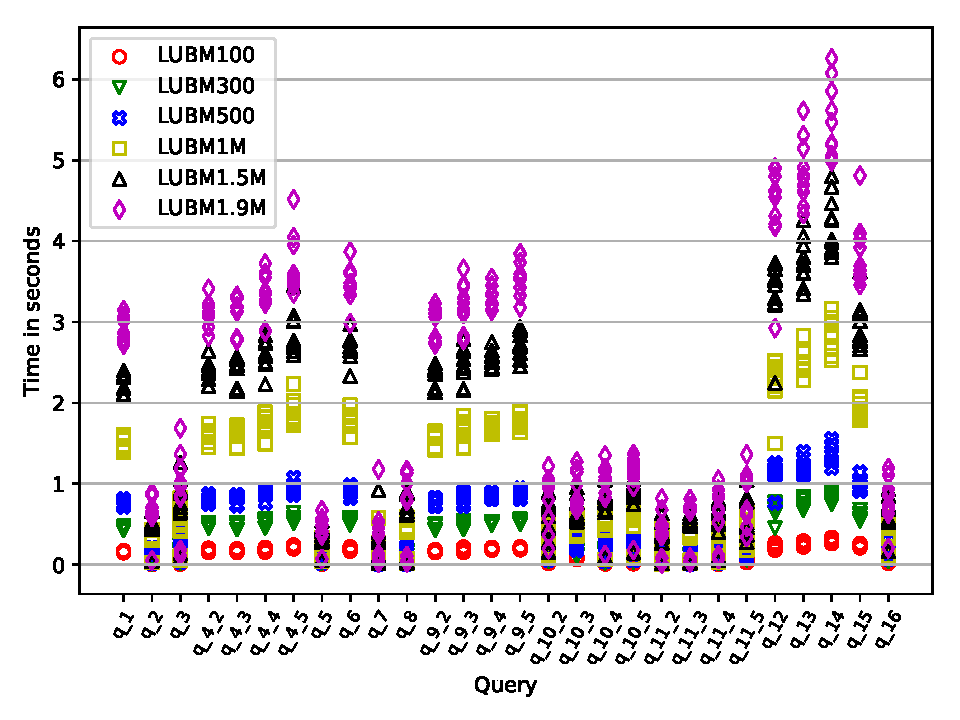
\includegraphics[width=0.48\textwidth]{data/LUBM_all.pdf}
   \caption{Reachability index creation time for LUBM graphs}
   \label{fig:lubm_all_qs}
\end{figure}

Reachability index creation time for each query for for real-world graphs is presented in figure~\ref{fig:other_all_qs}.
We can see that query evaluation time depends on graph inner structure. 
First of all, in some cases handling of small graph requires more time, then handling bigger graph.
For example, $Q_{10}^4$: querying the \textit{geospecies} graph (450k vertices) in some cases requires more time than querying of \textit{mappingbased\_properties} (8.3M vertices) and \textit{taxonomy} (5.7M vertices).
On the other hand, \textit{taxonomy} querying in relatively big number of cases requires significantly more time, than querying of other graphs, while \textit{taxonomy} is not a biggest graph. 
Finally, we can see, that in big number of cases query execution time requires less then 10 seconds, even for big graph, and no queries which require more then 52.17 seconds. 

\begin{figure}
   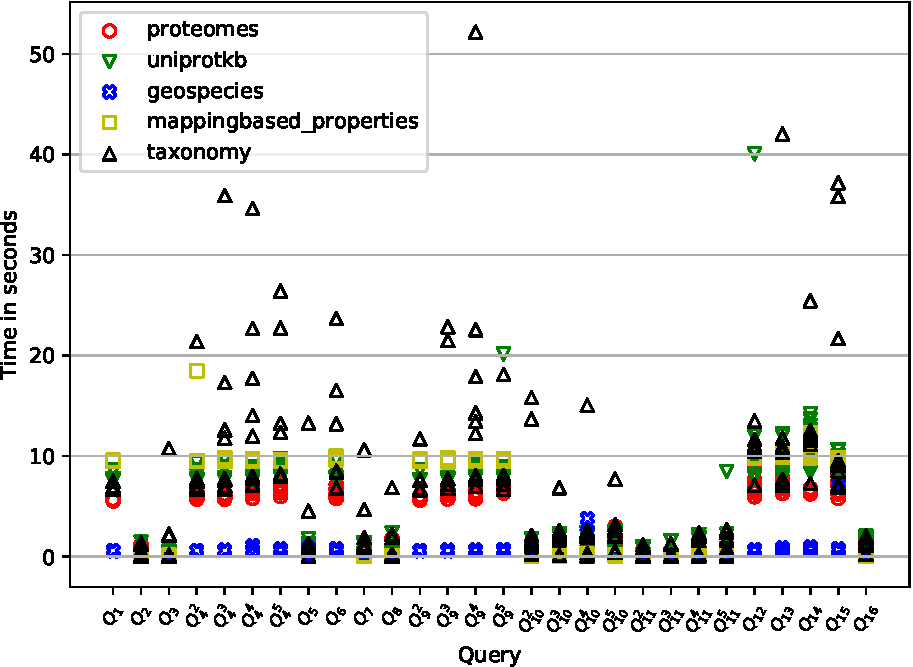
\includegraphics[width=0.48\textwidth]{data/other_all.pdf}
   \caption{Reachability index creation time for real-world RDFs}
   \label{fig:other_all_qs}
\end{figure}

Paths extraction was evaluated on cases with possible long paths.
These cases were selected during reachability index creation by using number of iterations in transitive closure evaluation.
For each selected graph and query we measure paths extraction time for each reachable pair, reachability index creation time is not included because exactly the same index, as calculated at the previous step, is used for paths extraction. 

We evaluate two scenarios.
The first one is a single path extraction.
In this case results are represented as a dependency of extraction time on extracted path length.
We can see linear !!!!

The second scenario is many paths extraction.
Here we limit a number of path to extract by !!! 
In this case results are represented as a dependency of extraction time on number of extracted paths.


\begin{figure}
     \begin{subfigure}[b]{0.24\textwidth}
         \centering
         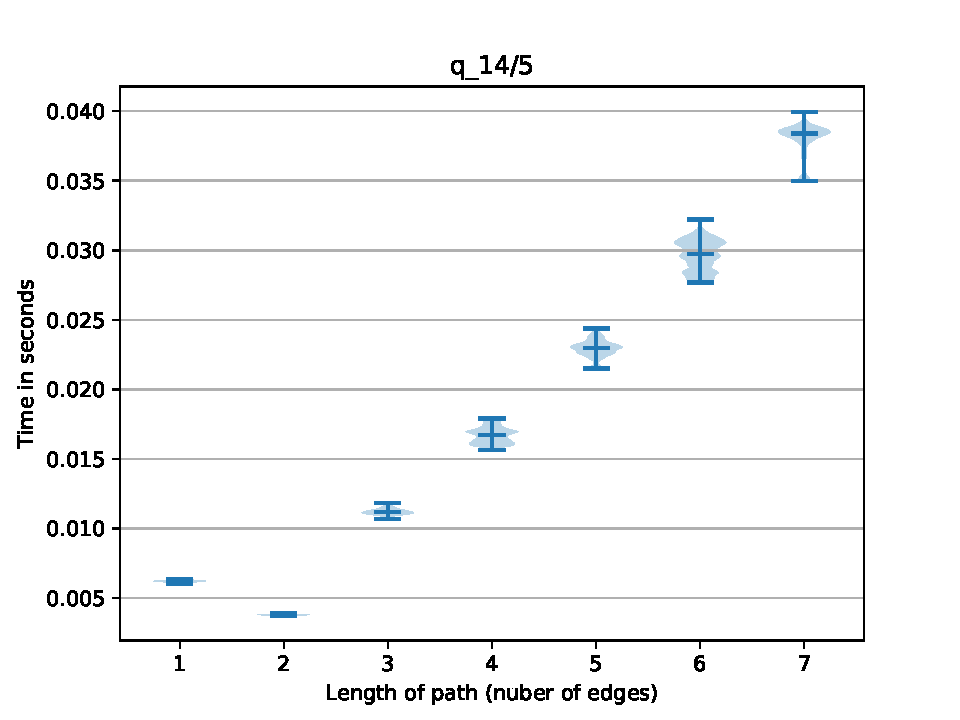
\includegraphics[width=\textwidth]{data/res_graphics/q_14_5.pdf}
         \caption{$y=x$}
         \label{fig:y equals x}
     \end{subfigure}
     ~\begin{subfigure}[b]{0.24\textwidth}
         \centering
         %\includegraphics[width=\textwidth]{data/res_graphics/q9_2_8.pdf}
         \caption{$y=x$}
         \label{fig:y equals x}
     \end{subfigure}\\
     \begin{subfigure}[b]{0.24\textwidth}
         \centering
         %\includegraphics[width=\textwidth]{data/res_graphics/q_14_8.pdf}
         \caption{$y=x$}
         \label{fig:y equals x}
     \end{subfigure}
     ~\begin{subfigure}[b]{0.24\textwidth}
         \centering
         %\includegraphics[width=\textwidth]{data/res_graphics/q4_2_8.pdf}
         \caption{$y=x$}
         \label{fig:y equals x}
     \end{subfigure}
   %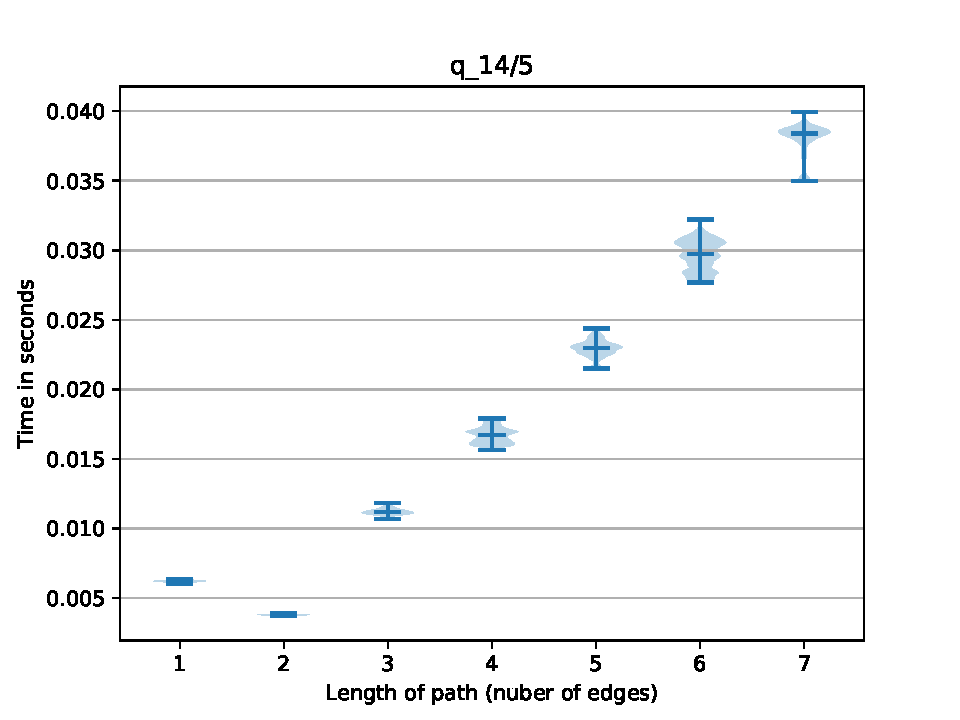
\includegraphics[width=0.48\textwidth]{data/res_graphics/q_14_5.pdf}
   \caption{Single path extraction}
\end{figure}

\subsubsection{Conclusion}

We can conclude that proposed algorithm is applicable for real-world data processing: the algorithm allows one both to solve reachability problem and to extract paths of interest in reasonable time even using na{\"i}ve implementation.  

\subsection{CFPQ Evaluation}

Comparison with matrix-based algorithm.

\subsubsection{Dataset}

Dataset for evaluation. 
It should be CFPQ\_Data\footnote{CFPQ\_Data is a dataset for CFPQ evaluation which contains both synthetic and real-world data and queries \url{https://github.com/JetBrains-Research/CFPQ\_Data}. Access date: 07.07.2020.}

\begin{table}
{
\rowcolors{2}{black!2}{black!10}
\begin{tabular}{|l|c|c|}
\hline
Graph & \#V & \#E \\
\hline
\hline 
eclass\_514en  & 120 926 & 484 646 \\
enzyme  & 358 434 & 144 9711 \\
geospecies  & 596 760 & 2 416 513 \\
go   & 1 188 340 & 4 820 728 \\
go-hierarchy & 1 780 956 & 7 228 358 \\
taxonomy & 2 308 385 & 9 369 511 \\
\hline
Aliases 1 & 6 442 630 & 24 465 430 \\
Aliases 2 & 4 834 262 & 12 366 973 \\
.... & 5 728 398 & 14 922 125 \\
\hline
\end{tabular}
}
\caption{Graphs for CFPQ evaluation}
\label{tbl:graphs_for_cfpq}
\end{table}



Same-generation queries, memory aliases.

\subsubsection{Results}

Results of evaluation.

Index creation.

{\setlength{\tabcolsep}{0.4em}
	\begin{table}
		\caption{RDFs query $G_1$ and $G_2$ (time is measured in seconds and memory is measured in megabytes)}
		\label{tbl:tableRDFQ1_appendix}
		\rowcolors{4}{black!2}{black!10}
		\small
		\begin{tabular}{| l | c | c | c | c |}
			\hline
			
			\multirow{2}{*}{Name}  & \multicolumn{2}{c|}{$G_1$} & \multicolumn{2}{c|}{$G_2$} \\
			\cline{2-5}
			                       & Tensors & RG\_CPU\textsubscript{path} & Tensors & RG\_CPU\textsubscript{path}	 \\
			\hline
			\hline
			eclass\_514en   & 0.254   & 0.195   & 0.227 & ...\\
			enzyme          & 0.035   & 0.029   & 0.036 & ...\\
			geospecies      & 0.091   & ...     & 0.001 & ...\\
			go-hierarchy    & 0.186   & 0.976   & 0.293 & ...\\
			go              & 1.676   & 1.286   & 1.368 & ...\\
			pathways        & 0.015   & 0.021   & 0.009 & ...\\
			taxonomy        & 5.366   & .....   & 3.282 & ...\\
			\hline
		\end{tabular}
	\end{table}
}


Paths extraction.

\subsubsection{Conclusion}

\section{Conclusion and future work}
In this paper, we shown how the context-free path query evaluation w.r.t. the relational and the single-path query semantics can be reduced to the calculation of matrix transitive closure. Also, we provided a formal proof of the correctness of the proposed reduction. In addition, we introduced an algorithm for computing this transitive closure, which allows us to efficiently apply GPGPU computing techniques. Finally, we shown the practical applicability of the proposed algorithm by running different implementations of our algorithm on real-world data.

We can identify several open problems for further research. In this paper we have considered only two semantics of context-free path querying but there are other important semantics, such as all-path query semantics~\cite{hellingsPathQuerying} which requires to present all paths for all triples $(A,m,n)$. Context-free path querying implemented with algorithm~\cite{GLL} can answer the queries in all-path query semantics by constructing a parse forest. It is possible to construct a parse forest for a linear input by matrix multiplication~\cite{okhotin_cyk}. Whether it is possible to generalize this approach for a graph input is an open question.

In our algorithm, we calculate the matrix transitive closure naively, but there are algorithms for the transitive closure calculation, which are asymptotically more efficient. Therefore, the question is whether it is possible to apply these algorithms for the matrix transitive closure calculation to the problem of context-free path querying.

Also, there are Boolean grammars~\cite{okhotinBoolean}, which have more expressive power than context-free grammars. Boolean path querying is an undecidable problem~\cite{hellingsRelational} but our algorithm can be trivially generalized to work on boolean grammars because parsing with boolean grammars can be expressed by matrix multiplication~\cite{okhotin_cyk}. It is not clear what a result of our algorithm applied to Boolean grammars would look like. Our hypothesis is that it would produce the upper approximation of a solution.

From a practical point of view, matrix multiplication in the main loop of the proposed algorithm may be performed on different GPGPU independently. It can help to utilize the power of multi-GPU systems and increase the performance of context-free path querying.

There is an algorithm~\cite{apspGPU} for transitive closure calculation on directed graphs which generalized to handle graph sizes inherently larger then the DRAM memory available on the GPU. Therefore, the question is whether it is possible to apply this approach to the matrix transitive closure calculation in the problem of context-free path querying.
\section*{Acknowledgments}

We are grateful to Dmitri Boulytchev, Ekaterina Verbitskaia, Marina Polubelova, Dmitrii Kosarev and Dmitry Koznov for their careful reading, pointing out some mistakes, and invaluable suggestions.
This work is supported by grant from JetBrains Research.

\bibliographystyle{ACM-Reference-Format}
\bibliography{graphparsing}

\end{document}
